% !TeX spellcheck = ru_RU
\documentclass[a4paper,12pt]{extarticle}
\usepackage[utf8x]{inputenc}
\usepackage[T1,T2A]{fontenc}
\usepackage[russian]{babel}
\usepackage{hyperref}
\usepackage{indentfirst}
\usepackage{listings}
\usepackage{color}
\usepackage{here}
\usepackage{array}
\usepackage{multirow}
\usepackage{graphicx}

\usepackage{caption}
\renewcommand{\lstlistingname}{Программа} % заголовок листингов кода

\bibliographystyle{ugost2008ls}

\usepackage{listings}
\lstset{ %
extendedchars=\true,
keepspaces=true,
language=C,						% choose the language of the code
basicstyle=\footnotesize,		% the size of the fonts that are used for the code
numbers=left,					% where to put the line-numbers
numberstyle=\footnotesize,		% the size of the fonts that are used for the line-numbers
stepnumber=1,					% the step between two line-numbers. If it is 1 each line will be numbered
numbersep=5pt,					% how far the line-numbers are from the code
backgroundcolor=\color{white},	% choose the background color. You must add \usepackage{color}
showspaces=false				% show spaces adding particular underscores
showstringspaces=false,			% underline spaces within strings
showtabs=false,					% show tabs within strings adding particular underscores
frame=single,           		% adds a frame around the code
tabsize=2,						% sets default tabsize to 2 spaces
captionpos=t,					% sets the caption-position to top
breaklines=true,				% sets automatic line breaking
breakatwhitespace=false,		% sets if automatic breaks should only happen at whitespace
escapeinside={\%*}{*)},			% if you want to add a comment within your code
postbreak=\raisebox{0ex}[0ex][0ex]{\ensuremath{\color{red}\hookrightarrow\space}},
texcl=true,
inputpath=listings,                     % директория с листингами
}

\usepackage[left=2cm,right=2cm,
top=2cm,bottom=2cm,bindingoffset=0cm]{geometry}

%% Нумерация картинок по секциям
\usepackage{chngcntr}
\counterwithin{figure}{section}
\counterwithin{table}{section}

%%Точки нумерации заголовков
\usepackage{titlesec}
\titlelabel{\thetitle.\quad}
\usepackage[dotinlabels]{titletoc}

%% Оформления подписи рисунка
\addto\captionsrussian{\renewcommand{\figurename}{Рисунок}}
\captionsetup[figure]{labelsep = period}

%% Подпись таблицы
\DeclareCaptionFormat{hfillstart}{\hfill#1#2#3\par}
\captionsetup[table]{format=hfillstart,labelsep=newline,justification=centering,skip=-10pt,textfont=bf}

%% Путь к каталогу с рисунками
\graphicspath{{fig/}}

%% Внесение titlepage в учёт счётчика страниц
\makeatletter
\renewenvironment{titlepage} {
 \thispagestyle{empty}
}
\makeatother

\usepackage{minted}

\begin{document}	% начало документа

% Титульная страница
\begin{titlepage}	% начало титульной страницы

	\begin{center}		% выравнивание по центру

		\large Санкт-Петербургский Политехнический Университет Петра Великого\\
		\large Институт компьютерных наук и технологий \\
		\large Кафедра компьютерных систем и программных технологий\\[6cm]
		% название института, затем отступ 6см
		
		\huge Базы данных\\[0.5cm] % название работы, затем отступ 0,5см
		\large Отчет по лабораторной работе №1\\[0.1cm]
		\large Разработка структуры БД\\[5cm]

	\end{center}


	\begin{flushright} % выравнивание по правому краю
		\begin{minipage}{0.25\textwidth} % врезка в половину ширины текста
			\begin{flushleft} % выровнять её содержимое по левому краю

				\large\textbf{Работу выполнил:}\\
				\large Графов Д.И.\\
				\large {Группа:} 33531/2\\
				
				\large \textbf{Преподаватель:}\\
				\large Мяснов А.В.

			\end{flushleft}
		\end{minipage}
	\end{flushright}
	
	\vfill % заполнить всё доступное ниже пространство

	\begin{center}
	\large Санкт-Петербург\\
	\large \the\year % вывести дату
	\end{center} % закончить выравнивание по центру

\thispagestyle{empty} % не нумеровать страницу
\end{titlepage} % конец титульной страницы

\vfill % заполнить всё доступное ниже пространство


\newpage
\setcounter{page}{2}
% Содержание
% Содержание
\renewcommand\contentsname{\centerline{Содержание}}
\tableofcontents
\newpage




\section{Цель работы}
Сформировать набор данных, позволяющий производить операции на реальных объемах данных.

\section{Программа работы}
	\begin {enumerate}
	\item Реализация в виде программы параметризуемого генератора, который позволит сформировать набор связанных данных в каждой таблице.
	\item Частные требования к генератору, набору данных и результирующему набору данных:
	\begin{itemize}
		\item количество записей в справочных таблицах должно соответствовать ограничениям предметной области
		\item количество записей в таблицах, хранящих информацию об объектах или субъектах должно быть параметром генерации
		\item значения для внешних ключей необходимо брать из связанных таблиц
	\end{itemize}
	\end {enumerate}

\section{Выполнение работы}
В качестве языка программирования для параметризуемого создания генератора был выбран Python 3.6 и библиотека psycopg2 - самая популярная библиотека для работы с PostgreSQL.

В ходе выполнения работы была написана программа, реализующая генератор.
Код программы приведён ниже.

\large {Листинг 1. fill.py}
\inputminted[
frame=lines,
framesep=2mm,
baselinestretch=1.2,
fontsize=\footnotesize,
linenos
]{python}{../src/fill.py}

\section {Результат работы}

Запустим данную программу через терминал.

\begin{lstlisting}
(base) grafa@KRAB:~/Desktop/wine_card/lab3/src$ python fill.py
Successfully filled components and drinks!
Successfully filled places!
Successfully filled food!
Successfully filled places_food!
Successfully filled places_drinks!
Successfully filled discounts!
Successfully filled supplies_drinks!
Successfully filled supplies_food!
\end{lstlisting}

Примеры генерируемых данных:

\begin{figure}[H]
	\begin{center}
		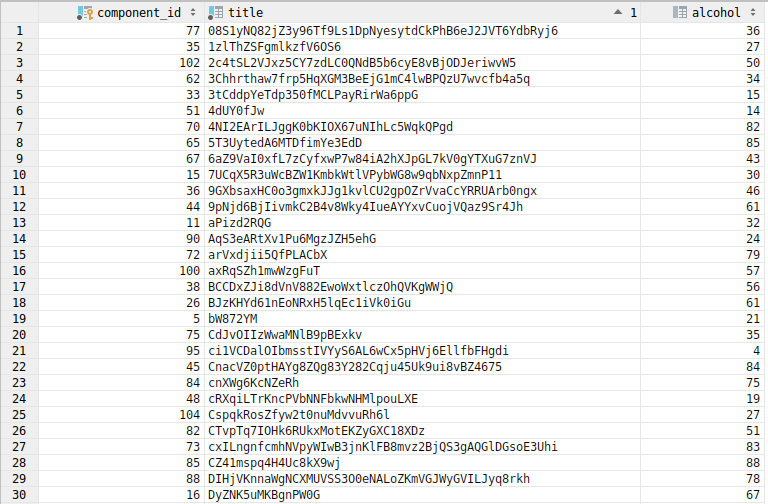
\includegraphics[scale=0.3]{./pics/components.png}
		\caption{Содержимое таблицы components} 
		\label{pic:components} % название для ссылок внутри кода
	\end{center}
\end{figure}

\begin{figure}[H]
	\begin{center}
		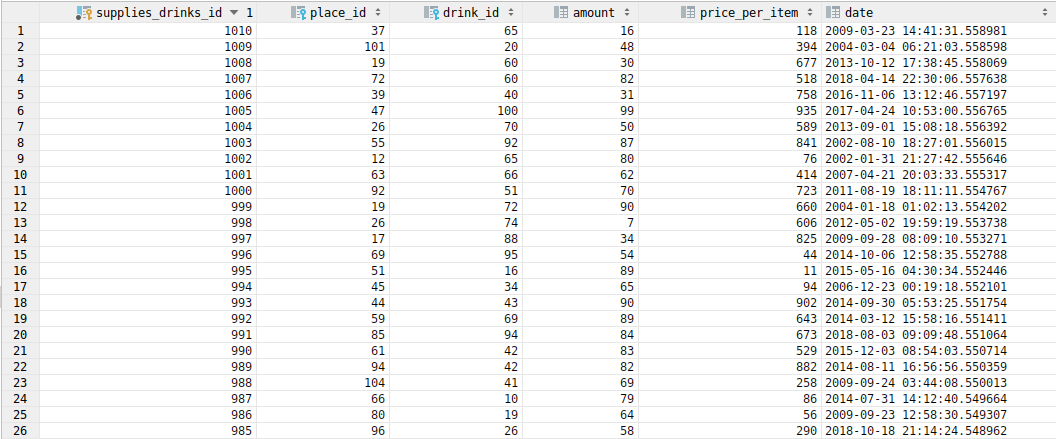
\includegraphics[scale=0.5]{./pics/supplies_drinks.png}
		\caption{Содержимое таблицы supplies\_drinks} 
		\label{pic:supplies_drinks} % название для ссылок внутри кода
	\end{center}
\end{figure}

\begin{figure}[H]
	\begin{center}
		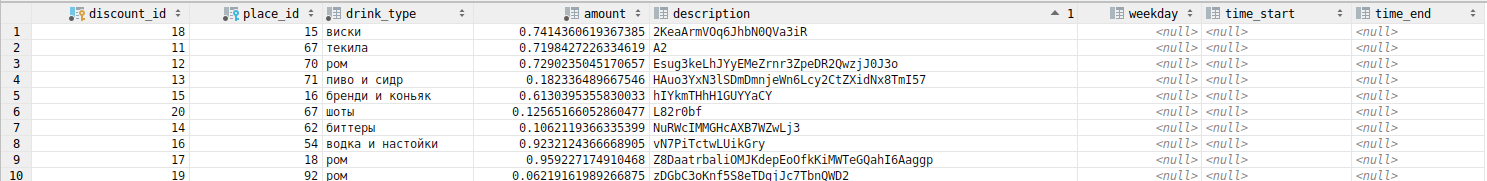
\includegraphics[scale=0.5]{./pics/discounts.png}
		\caption{Содержимое таблицы discounts} 
		\label{pic:discounts} % название для ссылок внутри кода
	\end{center}
\end{figure}


\newpage
\section{Выводы}

В ходе выполнения данной работы на языке программирования Python был написан параметризуемый генератор.
В качестве параметра данного генератора можно указать количество записей в таблицах, как это и требовало задание.
\end{document}

